
        \documentclass[a4paper,12pt]{article}
        \usepackage[utf8]{inputenc}
        \usepackage[brazil]{babel}
        \usepackage{geometry}
        \usepackage{array} % Para alinhamento vertical
        \usepackage{tabularx}
        \usepackage{graphicx}
        \usepackage{tikz}
        \usepackage{fancyhdr}
        \usepackage{multicol}

        \geometry{
            top=1.5cm,
            bottom=1.5cm,
            left=1.5cm,
            right=1.5cm
        }

        \newcommand{\opcao}[1]{%
            \tikz[baseline=-0.5ex]\draw (0,0) circle (0.25cm) node {#1};%
        }

        \newcommand{\opcaocorreta}[1]{%
            \tikz[baseline=-0.5ex]\filldraw[fill=black] (0,0) circle (0.25cm) node[white]{#1};%
        }

        \newcommand{\qrspace}[1][2cm]{%
            \begin{tikzpicture}
                \draw[thick] (0,0) rectangle (#1,#1);
                \node at (#1/2,#1/2) {\small QR CODE};
            \end{tikzpicture}%
        }

        \pagestyle{fancy}
        \fancyhf{}
        \renewcommand{\headrulewidth}{0pt}

        \begin{document}

        \begin{center}
            {\Large \textbf{CARTÃO DE RESPOSTA}}
        \end{center}

        \begin{tabularx}{\textwidth}{|>{\centering\arraybackslash}X|>{\centering\arraybackslash}m{4cm}|}
        \hline
        \textbf{DADOS DO CANDIDATO} & \textbf{QR CODE} \\
        \hline
        \begin{minipage}[c]{\linewidth}
        \hrulefill \\[0.3cm]
        \textbf{Nome: }RicardoFudido \\[0.3cm]
        \textbf{Matrícula:} \hrulefill \\[0.3cm]
        \textbf{Turma:} \hrulefill \\[0.3cm]
        \textbf{Data:} \hrulefill
        \end{minipage}
        &
        \begin{minipage}[c]{\linewidth}
        \centering
        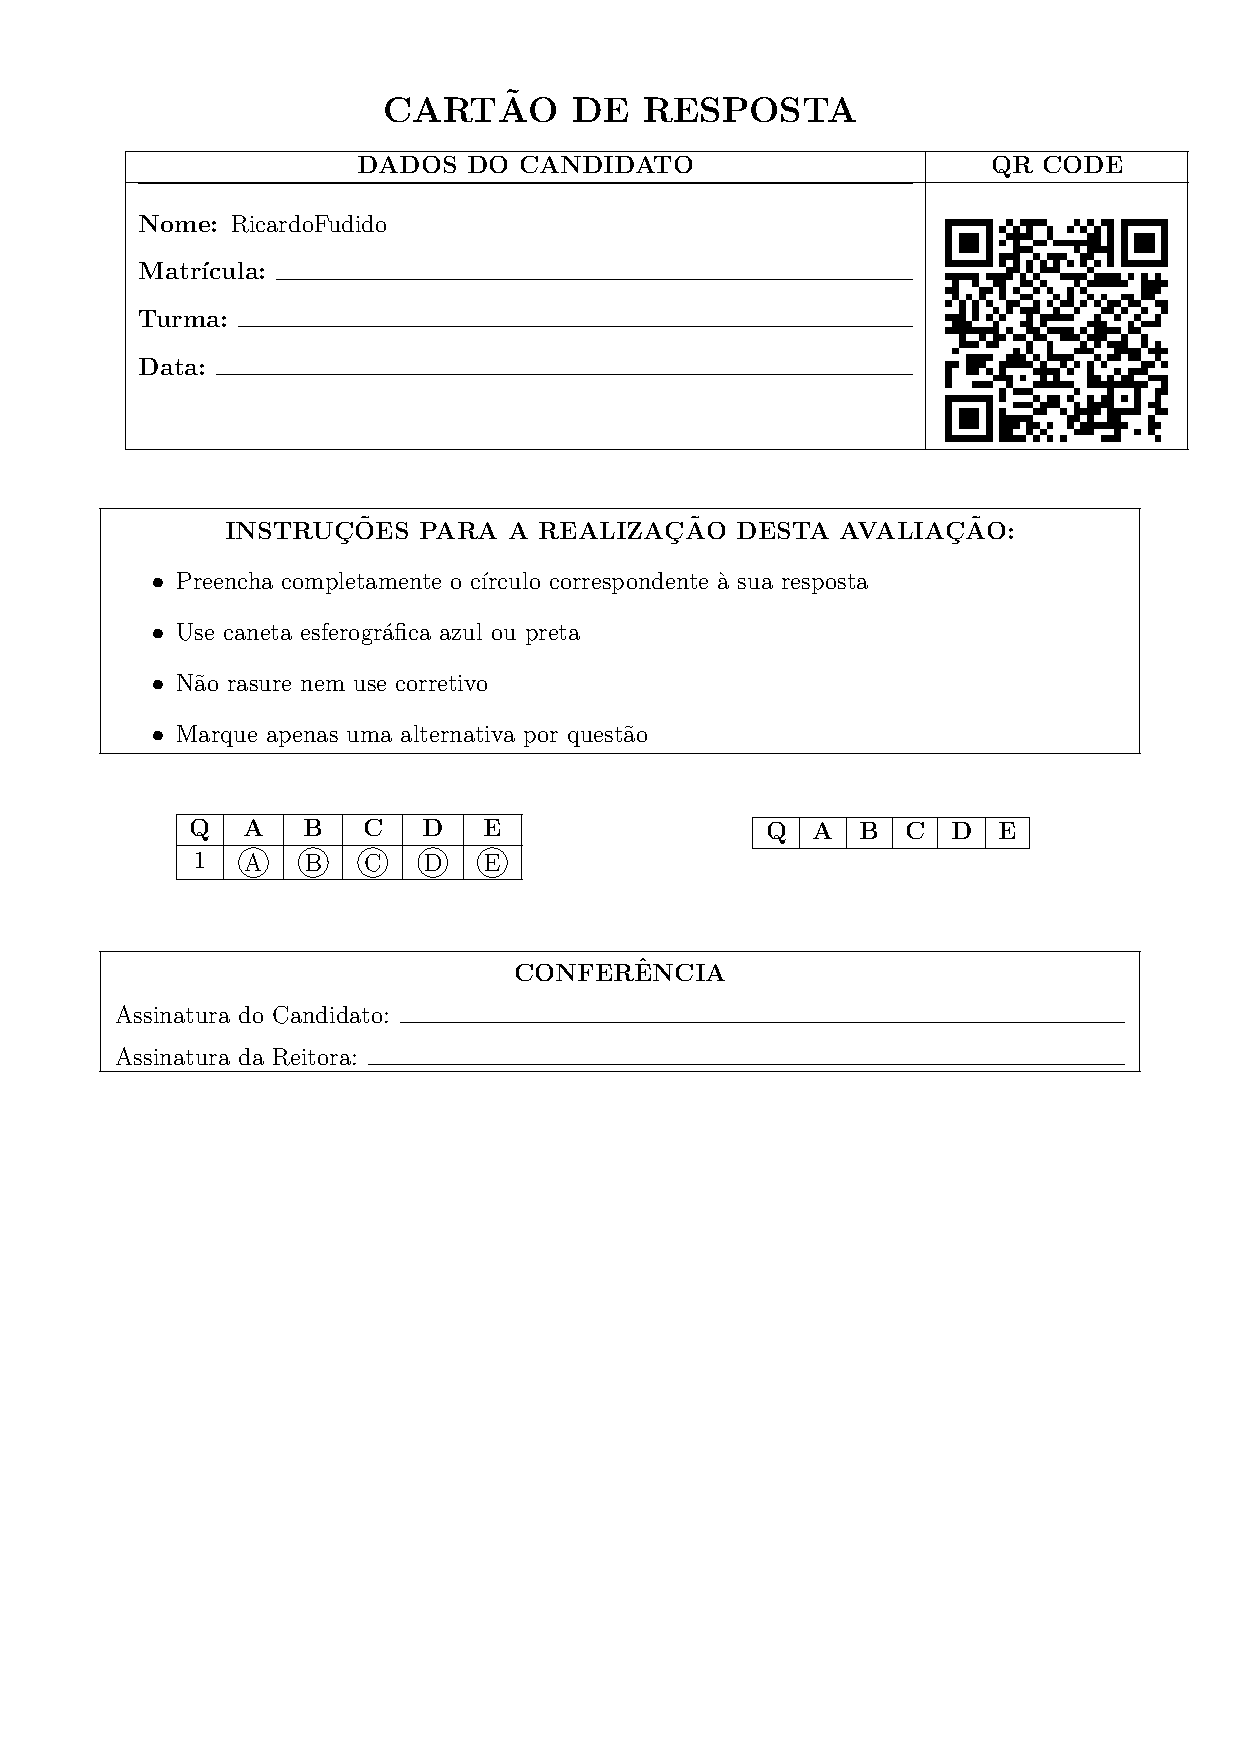
\includegraphics[width=4cm,height=4cm,keepaspectratio=false]{RicardoFudido.png}
        \end{minipage}
        \\
        \hline
        \end{tabularx}

        \vspace{0.5cm}

        \begin{center}
        \fbox{
        \begin{minipage}{0.95\textwidth}
            \centering
            \textbf{INSTRUÇÕES PARA A REALIZAÇÃO DESTA AVALIAÇÃO:}
            \begin{itemize}
                \item Preencha completamente o círculo correspondente à sua resposta
                \item Use caneta esferográfica azul ou preta
                \item Não rasure nem use corretivo
                \item Marque apenas uma alternativa por questão
            \end{itemize}
        \end{minipage}
        }
        \end{center}

        \vspace{0.5cm}

        % Primeira coluna de questões (1-1)
        \begin{multicols}{2}
        \begin{center}
        \begin{tabular}{|c|c|c|c|c|c|}
        \hline
        \textbf{Q} & \textbf{A} & \textbf{B} & \textbf{C} & \textbf{D} & \textbf{E} \\
        \hline
        1 & \opcao{A} & \opcao{B} & \opcao{C} & \opcao{D} & \opcao{E} \\
        \hline
        
        \end{tabular}
        \end{center}

        \columnbreak

        % Segunda coluna de questões (2-1)
        \begin{center}
        \begin{tabular}{|c|c|c|c|c|c|}
        \hline
        \textbf{Q} & \textbf{A} & \textbf{B} & \textbf{C} & \textbf{D} & \textbf{E} \\
        \hline
        
        \end{tabular}
        \end{center}
        \end{multicols}

        \vspace{0.5cm}

        % Rodapé com informações adicionais
        \begin{center}
        \fbox{
        \begin{minipage}{0.95\textwidth}
            \centering
            \textbf{CONFERÊNCIA}\\
            \vspace{0.2cm}
            Assinatura do Candidato: \hrulefill \\
            \vspace{0.2cm}
            Assinatura da Reitora: \hrulefill
        \end{minipage}
        }
        \end{center}

        \end{document}
        